%%%%%%%%%%%%%%%%%%%%%%%%%%%%%%%%%%%%%%%%%%%%%%%%%%%%%%%%%%%%%%%%%%%%%
%% This is a (brief) model paper using the achemso class
%% The document class accepts keyval options, which should include
%% the target journal and optionally the manuscript type.
%%%%%%%%%%%%%%%%%%%%%%%%%%%%%%%%%%%%%%%%%%%%%%%%%%%%%%%%%%%%%%%%%%%%%
\documentclass[journal=jacsat,manuscript=article]{achemso}

%%%%%%%%%%%%%%%%%%%%%%%%%%%%%%%%%%%%%%%%%%%%%%%%%%%%%%%%%%%%%%%%%%%%%
%% Place any additional packages needed here.  Only include packages
%% which are essential, to avoid problems later. Do NOT use any
%% packages which require e-TeX (for example etoolbox): the e-TeX
%% extensions are not currently available on the ACS conversion
%% servers.
%%%%%%%%%%%%%%%%%%%%%%%%%%%%%%%%%%%%%%%%%%%%%%%%%%%%%%%%%%%%%%%%%%%%%
\usepackage[version=3]{mhchem} % Formula subscripts using \ce{}

%%%%%%%%%%%%%%%%%%%%%%%%%%%%%%%%%%%%%%%%%%%%%%%%%%%%%%%%%%%%%%%%%%%%%
%% If issues arise when submitting your manuscript, you may want to
%% un-comment the next line.  This provides information on the
%% version of every file you have used.
%%%%%%%%%%%%%%%%%%%%%%%%%%%%%%%%%%%%%%%%%%%%%%%%%%%%%%%%%%%%%%%%%%%%%
%%\listfiles

%%%%%%%%%%%%%%%%%%%%%%%%%%%%%%%%%%%%%%%%%%%%%%%%%%%%%%%%%%%%%%%%%%%%%
%% Place any additional macros here.  Please use \newcommand* where
%% possible, and avoid layout-changing macros (which are not used
%% when typesetting).
%%%%%%%%%%%%%%%%%%%%%%%%%%%%%%%%%%%%%%%%%%%%%%%%%%%%%%%%%%%%%%%%%%%%%
\newcommand*\mycommand[1]{\texttt{\emph{#1}}}

%%%%%%%%%%%%%%%%%%%%%%%%%%%%%%%%%%%%%%%%%%%%%%%%%%%%%%%%%%%%%%%%%%%%%
%% Meta-data block
%% ---------------
%% Each author should be given as a separate \author command.
%%
%% Corresponding authors should have an e-mail given after the author
%% name as an \email command. Phone and fax numbers can be given
%% using \phone and \fax, respectively; this information is optional.
%%
%% The affiliation of authors is given after the authors; each
%% \affiliation command applies to all preceding authors not already
%% assigned an affiliation.
%%
%% The affiliation takes an option argument for the short name.  This
%% will typically be something like "University of Somewhere".
%%
%% The \altaffiliation macro should be used for new address, etc.
%% On the other hand, \alsoaffiliation is used on a per author basis
%% when authors are associated with multiple institutions.
%%%%%%%%%%%%%%%%%%%%%%%%%%%%%%%%%%%%%%%%%%%%%%%%%%%%%%%%%%%%%%%%%%%%%
\author{Jiaqi He}
\altaffiliation{These authors contributed equally to this work.}
\affiliation
{Key Laboratory of Luminescence and Optical Information, Ministry of Education, Institute of Optoelectronic Technology, Beijing Jiaotong University, Beijing 100044, China}
\alsoaffiliation{Guangxi Colleges and Universities Key Laboratory of Microwave and Optical Wave-Applied Technology, Guilin 541004, China}

\author{Taishen Li}
\affiliation{Hefei National Laboratory for Physical Sciences at the Microscale, University of Science and Technology of China, Hefei 230026, China}
\altaffiliation{These authors contributed equally to this work.}

\author{Lu Zhang}
\affiliation
{Key Laboratory of Luminescence and Optical Information, Ministry of Education, Institute of Optoelectronic Technology, Beijing Jiaotong University, Beijing 100044, China}

\author{Dawei He}
\email{dwhe@bjtu.edu.cn}
\phone{+86 (0)10 51688018}
\affiliation
{Key Laboratory of Luminescence and Optical Information, Ministry of Education, Institute of Optoelectronic Technology, Beijing Jiaotong University, Beijing 100044, China}

\author{Yongsheng Wang}
\affiliation
{Key Laboratory of Luminescence and Optical Information, Ministry of Education, Institute of Optoelectronic Technology, Beijing Jiaotong University, Beijing 100044, China}

\author{Huaiyi Ding}
\email{dinghy@ustc.edu.cn}
\affiliation
{Hefei National Laboratory for Physical Sciences at the Microscale, University of Science and Technology of China, Hefei 230026, China}

\author{Nan Pan}
\affiliation
{Hefei National Laboratory for Physical Sciences at the Microscale, University of Science and Technology of China, Hefei 230026, China}

\author{Hui Zhao}
\affiliation{Department of Physics and Astronomy, University of Kansas, Lawrence, Kansas 66045, United States}

%%%%%%%%%%%%%%%%%%%%%%%%%%%%%%%%%%%%%%%%%%%%%%%%%%%%%%%%%%%%%%%%%%%%%
%% The document title should be given as usual. Some journals require
%% a running title from the author: this should be supplied as an
%% optional argument to \title.
%%%%%%%%%%%%%%%%%%%%%%%%%%%%%%%%%%%%%%%%%%%%%%%%%%%%%%%%%%%%%%%%%%%%%
\title[An \textsf{achemso} demo]
  {Efficient Energy Transfer in In$_2$Se$_3$-MoSe$_2$ van der Waals Heterostructures}

%%%%%%%%%%%%%%%%%%%%%%%%%%%%%%%%%%%%%%%%%%%%%%%%%%%%%%%%%%%%%%%%%%%%%
%% Some journals require a list of abbreviations or keywords to be
%% supplied. These should be set up here, and will be printed after
%% the title and author information, if needed.
%%%%%%%%%%%%%%%%%%%%%%%%%%%%%%%%%%%%%%%%%%%%%%%%%%%%%%%%%%%%%%%%%%%%%

\keywords{van der Waals heterostructure, two-dimensional material, energy transfer, ultrafast dynamics}

\begin{document}
%%%%%%%%%%%%%%%%%%%%%%%%%%%%%%%%%%%%%%%%%%%%%%%%%%%%%%%%%%%%%%%%%%%%%
%% The manuscript does not need to include \maketitle, which is
%% executed automatically.  The document should begin with an
%% abstract, if appropriate.  If one is given and should not be, the
%% contents will be gobbled.
%%%%%%%%%%%%%%%%%%%%%%%%%%%%%%%%%%%%%%%%%%%%%%%%%%%%%%%%%%%%%%%%%%%%%
\begin{abstract}
We show that bilayer $\alpha$-phase In$_2$Se$_3$ and monolayer MoSe$_2$ form a type-I band alignment, with both the conduction band minimum and the valance band maximum located in MoSe$_2$. Samples were fabricated by a two-step chemical vapor deposition method. The photoluminescence yield of the heterostructure sample was found to be similar to monolayer MoSe$_2$, indicating the lack of efficient charge transfer from MoSe$_2$ to In$_2$Se$_3$. This is further confirmed by the observation that the photocarrier lifetime in the heterostructure is similar to monolayer MoSe$_2$, showing the lack of layer separation of the electrons and holes. Efficient energy transfer from In$_2$Se$_3$ to MoSe$_2$ was observed by the 7-fold enhancement of the differential reflection signal in the heterostructure and its ultrashort rising time. Furthermore, we observed significant photoluminescence quenching in heterostructures formed by bulk In$_2$Se$_3$ and monolayer MoSe$_2$, which suggests efficient charge transfer and therefore type-II band alignment. These findings suggest that $\alpha$-In$_2$Se$_3$ ultrathin layers can be effectively integrated as light-absorbing layers with other transition metal dichalcogenides for novel optoelectronic applications.
\end{abstract}

%%%%%%%%%%%%%%%%%%%%%%%%%%%%%%%%%%%%%%%%%%%%%%%%%%%%%%%%%%%%%%%%%%%%%
%% Start the main part of the manuscript here.
%%%%%%%%%%%%%%%%%%%%%%%%%%%%%%%%%%%%%%%%%%%%%%%%%%%%%%%%%%%%%%%%%%%%%
\section{Introduction}

Since 2010, significant efforts have been devoted to studies of two-dimensional (2D) materials beyond graphene \cite{n522274,nn7699,2dm3042001}, such as transition metal dichalcogenides (TMDs) and phosphorene. These new materials possess several attractive features, including their layer-dependent electronic structures \cite{nl101271,l105136805} and crystal symmetry \cite{b87161403,nl133329}, the enhanced Coulomb interaction due to reduced dielectric screening \cite{l113076802,l113026803}, large optical absorption coefficients due to the van Hove singularity \cite{s3401311,apl105201905}, and being flexible \cite{nn8100}. Based on these novel properties, 2D materials have been considerred good candidates for applications such as field-effect transistors \cite{nn6147,nm12815}, integrated circuits \cite{nl124674}, solar cells\cite{nn9262}, photodetectors \cite{nn9262}, and light-emitting diodes \cite{s344725,nn9268,nn9257}. 

Recently, a relatively less explored 2D material, $\alpha$-phase In$_2$Se$_3$, has emerged as a promising material for novel optoelectronic applications. Unlike most TMDs that undergo an indirect-to-direct bandgap transition from bulk to monolayer (1L), reports have shown that $\alpha$-In$_2$-Se$_3$ may possess direct bandgaps in all thickness \cite{aom41939}. This could facilitate efficient light absorption and emission, which are beneficial for many optoelectronic applications. Furthermore, its bandgap changes from about 1.45 eV in bulk form to about 2.8 eV in few-layers \cite{aom41939}. Such a range is among the largest in 2D materials, and allows tuning of the operation wavelength of optoelectronic devices by thickness. Recently, several groups have reported high-gain and high-detectivity photodetectors of multilayer $\alpha$-In$_2$-Se$_3$ that perform better than most known 2D materials \cite{nl157853,acsnano8514,nl156400}. Demonstration of growth of high-quality monolayers by physical vapor deposition \cite{nl156400} also indicates potentials of large-scale production.

One advantage the 2D materials for optoelectronic applications is that they allow fabrication of multilayer heterostructures with tailored properties \cite{n499419}. These multilayers are bond by van der Waals interlayer coupling, which does not have individual atomic correspondence. Hence, the lattice matching requirement, which has been a major constrain when fabricating heterostructures with ionic or covalence materials, is largely relaxed. This new approach can thus produce a vast number of new materials, and can potentially transform material discovery \cite{nrm116042,s353461}. For example, heterostructures combining graphene and TMDs can improve performance of photodetectors \cite{nn8952,acsnano108252,nc713278} and photovoltaic devices \cite{s3401311,nn8952}. Combing different TMD monolayers can provide tuning of the optical and transport properties of these materials \cite{nc67666,pnas1116198,nl17938,nl164831} and control of photocarrier dynamics \cite{nn9682,acsnano812717,nc66242,nl175229,nn9676,nl17638}.

In this context, it is interesting to explore integration of In$_2$Se$_3$ with other 2D materials, such as TMDs. The effort will also expand the horizon of van der Waals heterostructures by introducing new materials with different lattice structures. Here we report a study on two key issues for developing such heterostructures, the nature of the band alignment and the interlayer energy and charge transfer. Understanding the band alignment is the first step to developing strategies to tailor the electronic and optical properties of these materials, while efficient energy or charge transfer is highly desired for harnessing emergent properties of 2D heterostructrues.

\section{Experimental}

The samples were fabricated by a two-step chemical vapor deposition (CVD) technique \cite{cjcp30325}. First, 1L MoSe$_2$ were synthesized on a SiO$_2$/Si substrate. As precursors, elemental Se and MoO$_3$ powders were put in zone 1 and zone 2 of a two-zone furnace. The substrate was located near MoO$_3$. Zone 1 and zone 2 were heated to 100 and 780$^\circ$C, respectively, in 15 minutes. Then zone 1 was heated further to 270$^\circ$C in 5 minutes and kept for 30 minutes, with zone 2 kept at  780$^\circ$C. The reaction was under 40 sccm Ar and 10 sccm H$_2$ atmosphere. In the second step, In$_2$Se$_3$ were grown on the substrate with 1L MoSe$_2$. Se and In$_2$O$_3$ powders were used as the precursors. Other conditions were kept the same as for MoSe$_2$, except that the temperature of zone 2 was reduced to 660$^\circ$C and was kept for 25 minutes. 

\begin{figure}
  \centering
  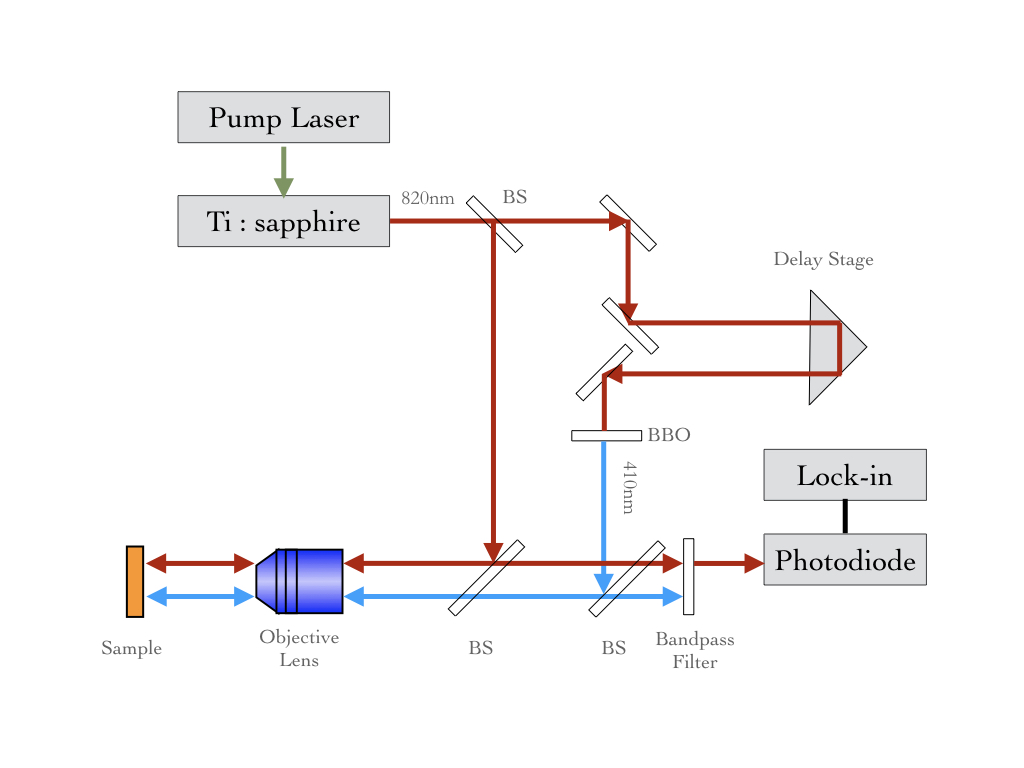
\includegraphics[width=9cm]{Setup.jpeg}
  \caption{Schematics of the experimental setup for differential reflection measurements.}
    \label{fig:tam}
\end{figure}

Time-resolved differential reflection measurements were performed with a setup that is schematically shown in Figure \ref{fig:tam}. A Ti:sapphire laser generates 100-fs pulses with a repetition rate of 80 MHz. The central wavelength of the pulse is 820 nm, with a full width at half maximum (FWHM) of about 10 nm. The 820-nm beam is split to 2 parts with a beamspilter. One part serves as the probe pulse while the other is focused to a beta barium borate crystal to generate its second harmonic at 410 nm, serving as the pump. The two beams are combined with a beamspliter and focused to the sample through a microscope objective lens. The sizes of the pump and probe spots are 1.5 and 2.5 $\mu$m in FWHM, respectively. The reflected probe is collected by the same lens and is sent to a silicon photodiode. A set of filters is put in front of photodiode to block the reflected pump beam. The output of photodiode is measured by a lock-in amplifier. A mechanical chopper is placed in the pump beam to modulate its intensity at about 2 KHz. All the measurements were taken at room temperature with samples exposed in air. With this configuration, the lock-in amplifier measures the differential reflection, $\Delta R / R_0 = (R - R_0) / R_0$, where $R$ and $R_0$ are the reflection coefficient of the probe with and without the presence of the pump beam, respectively \cite{afm271604509}.
\section{Results and discussion}

Presently, the nature of the band alignment between 2L In$_2$Se$_3$ and 1L MoSe$_2$ is still unclear. Kelvin probe force microscope measurements have shown that the difference of the Fermi levels between 2L In$_2$Se$_3$ and 1L MoSe$_2$ is only about 200 meV \cite{cjcp30325}. Since each Fermi level is near the bottom of the conduction band \cite{2dm4035019} and the bandgap of 2L In$_2$Se$_3$ is about 2.8 eV \cite{aom41939}, much larger than the optical bandgap of 1L MoSe$_2$ of 1.55 eV, it is safe to assume that the valance band maximum (VBM) of MoSe$_2$ is higher than In$_2$Se$_3$ by a large amount. However, the sign of the conduction band offset is unknown. If the conduction band minimum (CBM) of 1L MoSe$_2$ is lower than 2L In$_2$Se$_3$, as shown in Figure \ref{fig:alignment}(a), the heterostructure would be of type-I nature. In this case, one would expect energy transfer from In$_2$Se$_3$ to MoSe$_2$, (indicated by the arrow) {\it via} either Dexter or F{\"o}rster mechanisms. Neither charge transfer nor energy transfer would occur from MoSe$_2$ to In$_2$Se$_3$. On the other hand, a type-II heterostructure could form if the CBM of MoSe$_2$ is higher than In$_2$Se$_3$, as shown in Figure \ref{fig:alignment}(b). Such a band alignment would facilitate charge transfer, {\it i.e.} electron transfer from MoSe$_2$ to In$_2$Se$_3$, as indicated by the dashed arrow,  and hole transfer from In$_2$Se$_3$ to MoSe$_2$ (not shown). 

In the following discussions, we will show that the band alignment is type-I, and that the energy transfer from In$_2$Se$_3$ to MoSe$_2$ is ultrafast and highly efficient.

\begin{figure}
  \centering
  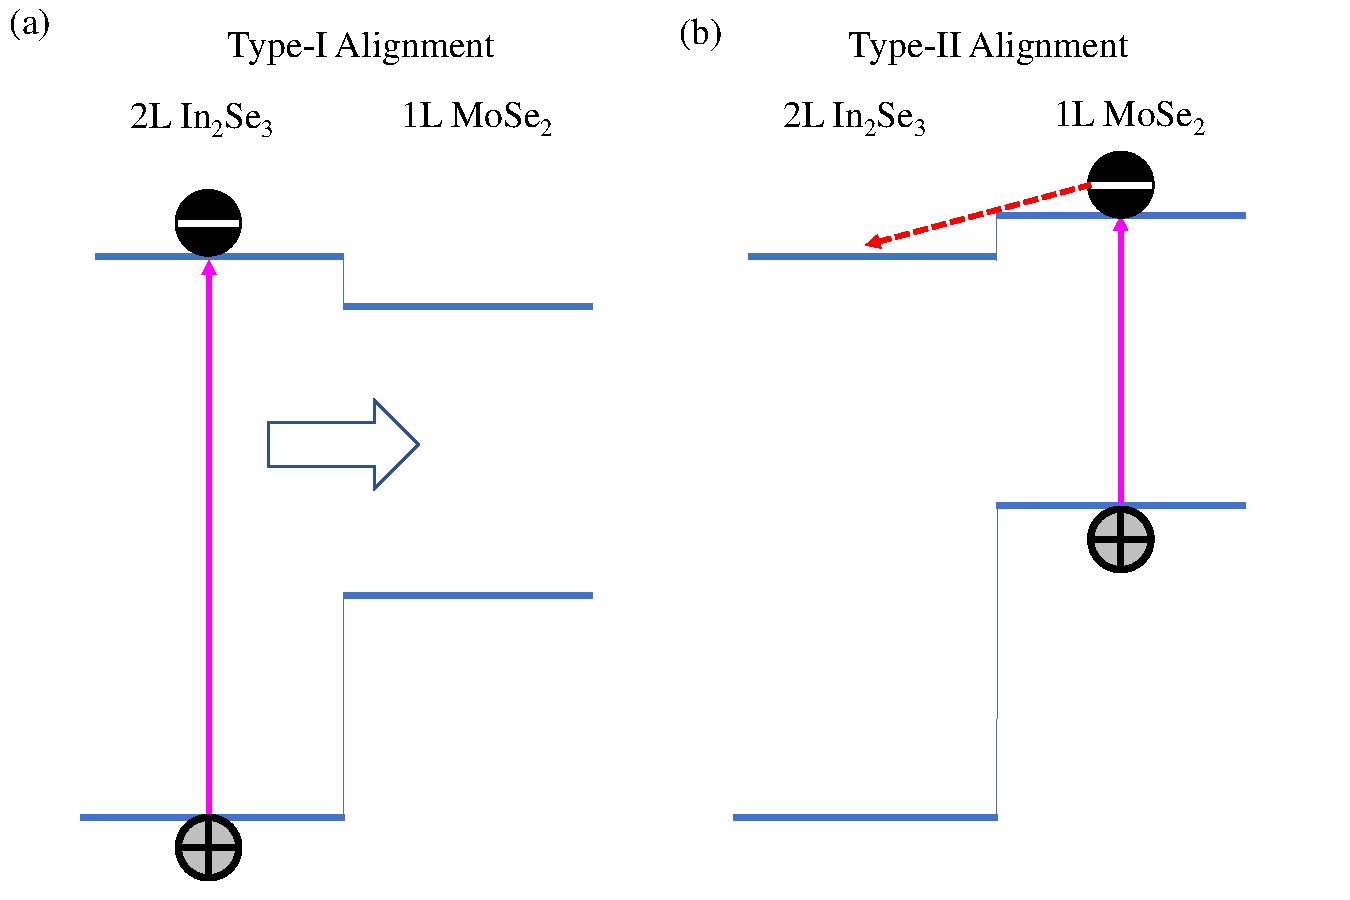
\includegraphics[width=9cm]{alignment.pdf}
  \caption{Possible band alignment of the 2L-In$_2$Se$_3$/1L-MoSe$_2$ heterostructure, showing type-I (a) and type-II (b) alignments with energy and charge transfers in each case.}
    \label{fig:alignment}
\end{figure}

Figure \ref{fig:sample}(a) shows the atomic model of the In$_2$Se$_3$-MoSe$_2$  heterostructures studied here, which were fabricated by chemical vapor deposition (CVD) \cite{cjcp30325} (see Experimental). Figure \ref{fig:sample}(b) shows optical microscope images of the 1L MoSe$_2$ (left panel) and the heterostructure samples (right panel). Since the flakes are on Si-SiO$_2$ substrates, the interference of multiple reflections results in different colors and contrasts of the two samples, which allow us to safely identify the samples. The identification  procedure has also been confirmed by atomic force microscopy measurements  \cite{cjcp30325}.

\begin{figure*}
  \centering
  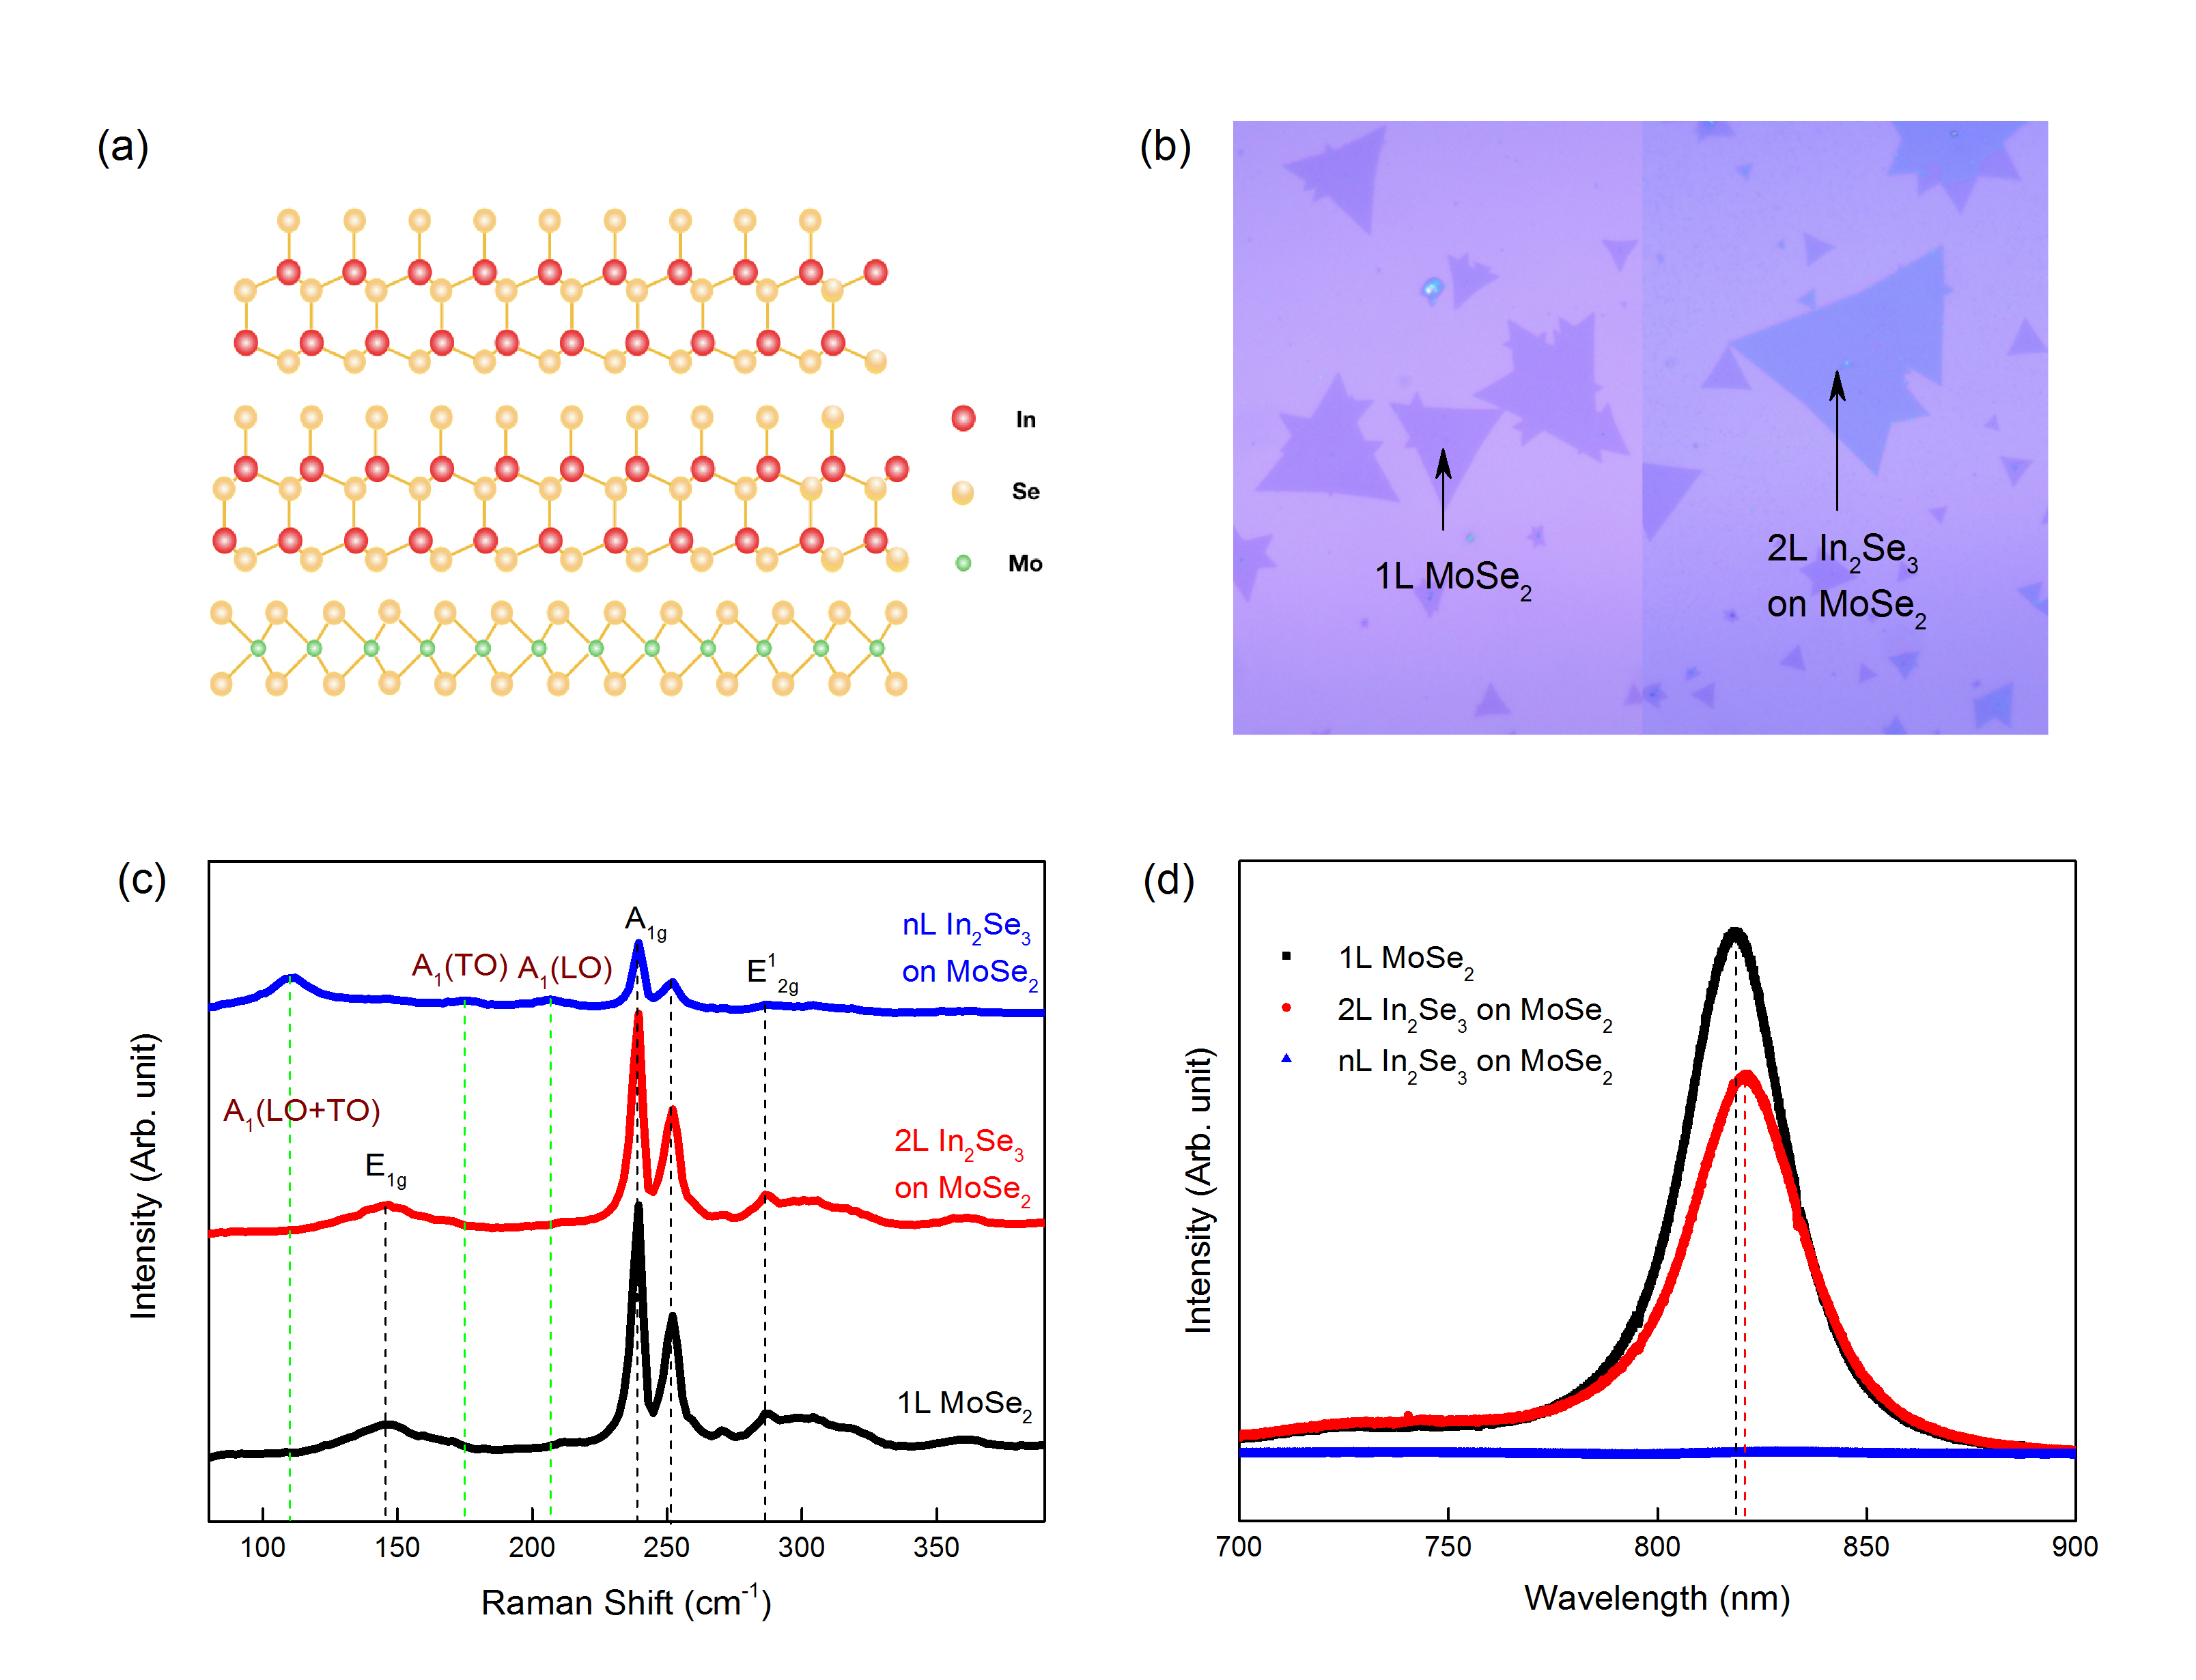
\includegraphics[width=14cm]{sample.jpg}
  \caption{(a) Schematic of the heterostructure sample formed by bilayer (2L) In$_2$Se$_3$ on monolayer (1L) MoSe$_2$. (b) Optical microscope images of the MoSe$_2$ 1L (left) and the heterostructure (right) on a Si/SiO$_2$ substrate. (c) Raman spectra of 1L MoSe$_2$, 2L In$_2$Se$_3$ on 1L MoSe$_2$, and bulk (nL) In$_2$Se$_3$ on 1L MoSe$_2$ obtained under the same condition. (d) Photoluminescence spectra of 1L MoSe$_2$, 2L In$_2$Se$_3$ on 1L MoSe$_2$, and bulk (nL) In$_2$Se$_3$ on 1L MoSe$_2$  obtained under the same condition.}
    \label{fig:sample}
\end{figure*}

The samples were characterized by Raman spectroscopy with a 532-nm laser. The black curve in Figure \ref{fig:sample}(c) shows the Raman spectrum obtained from a 1L-MoSe$_2$ flake. Four peaks are clearly observed, which are assigned to the E$_{1g}$ (about 145 cm$^{-1}$), A$_{1g}$ (about 239 cm$^{-1}$), E$_{2g}$ (about 286 cm$^{-1}$), and defect modes (about 252 cm$^{-1}$, respectively, according to previous reports \cite{oe214908,nanoscale64915}. The Raman spectrum measured from a heterostructure formed by bulk In$_2$Se$_3$ and 1L MoSe$_2$ is shown as the blue curve in Figure \ref{fig:sample}(c). We observed three peaks at about 110, 174, and 207  cm$^{-1}$. These peaks are reasonably consistent with previous reports of Raman spectra of $\alpha$-In$_2$Se$_3$ \cite{nl175508,nl156400}, and can be assigned to  A$_1$(LO+TO), A$_1$(TO) and A$_1$(LO) modes, respectively. Raman peaks from the underneath 1L MoSe$_2$ are reduced, but still visible, with no apparent shifts. The red curve in Figure \ref{fig:sample}(c) shows the Raman spectrum from the heterostructure formed by 2L In$_2$Se$_3$ and 1L MoSe$_2$. The In$_2$Se$_3$ peaks are greatly reduced, due to the smaller thickness, while the peaks from MoSe$_2$ are similar to the 1L-MoSe$_2$ sample. It has been well established that the width of these phonon modes in TMDs is sensitive to charge density, and broadens noticeably when the charge density is changed due to doping or interlayer charge transfer \cite{am262857,nanoscale919360}. The lack of broadening of these modes appears to suggest that the charge transfer in these heterostructures is insignificant. Furthermore, since the lattice strain often results in red-shift of these phonon modes \cite{b85161403,b88121301,nanoscale919360}, the absence of such shifts further confirms the strain-free growth of the heterostructures.

We next probe the potential charge and energy transfer processes in the heterostructures by comparing their photoluminescence (PL) with 1L MoSe$_2$. The black curve in Figure \ref{fig:sample}(d) shows the PL spectrum of 1L MoSe$_2$ under the excitation of a 532-nm continuous-wave laser. The spectrum and the PL yield are consistent with previous results \cite{oe214908,nanoscale64915}. With the same experimental conditions, the PL peak from the 2L-In$_2$Se$_3$/1L-MoSe$_2$ heterostructure (red curve) is similar to 1L MoSe$_2$. The small decrease of the intensity can be attributed to the additional loss when the excitation laser beam and the PL goes through the In$_2$Se$_3$ layer. The slight shift (from 819 to 821 nm) could be attributed to the effect of different dielectric environment on the optical bandgap of 1L MoSe$_2$. On the contrary, the heterostructure formed by bulk In$_2$Se$_2$ and 1L MoSe$_2$ shows no detectable PL under the same experimental conditions, as shown by the blue curve in Figure \ref{fig:sample}(d).

The lack of PL quenching in the 2L-In$_2$Se$_3$/1L-MoSe$_2$ heterostructure suggests that interlayer charge transfer in insignificant, which suggests that 2L In$_2$Se$_3$ and 1L MoSe$_2$ do not form a type-II band alignment. In type-II heterostructures formed by 2D materials, PL quenching induced by efficient charge transfer has been generally observed \cite{nc66242,pnas1116198,nn9676,nl144785,nl143185,acsnano96459,nanoscale717523,acsnano106612}.  The separation of the electrons and holes to the two layers suppresses their radiative recombination in either layer. In the PL measurement of 2L-In$_2$Se$_3$/1L-MoSe$_2$ heterostructure, the 532-nm laser only injects electrons and holes in MoSe$_2$, since its photon energy is smaller than the optical bandgap of 2L In$_2$Se$_3$. If the band alignment were type-II, electrons would transfer to In$_2$Se$_3$, as illustrated in Figure \ref{fig:alignment}(b), instead of radiatively recombining with the holes in MoSe$_2$. This process would induce significant quenching of MoSe$_2$ PL, in comparison to 1L MoSe$_2$ samples.

One alternative explanation of the lack of charge transfer is poor interface quality of the heterostructure samples. In manually stacked heterostructures, interface contamination could be introduced during the fabrication process, which can prevent interlayer charge transfer. However, the In$_2$Se$_3$ layer was directly grown on MoSe$_2$ by CVD. Hence, the interface is expected to be free of contamination. Indeed, the significant PL quenching in nL-In$_2$Se$_3$/1L-MoSe$_2$ heterostructure confirms the high quality of the interface between MoSe$_2$ and In$_2$Se$_3$. Since nL In$_2$Se$_3$ has a much smaller bandgap than 2L In$_2$Se$_3$, it is very likely that it forms type-II alignment with 1L MoSe$_2$. Since the interface quality between nL In$_2$Se$_3$ and 1L MoSe$_2$ is high enough to allow such efficient charge transfer, the interface of the 2L-In$_2$Se$_3$/1L-MoSe$_2$ samples obtained during the same fabrication procedure should have comparable quality. Hence, the lack of charge transfer is most likely due to a type-I band alignment as illustrated in Figure \ref{fig:alignment}(a).

\begin{figure*}
  \centering
  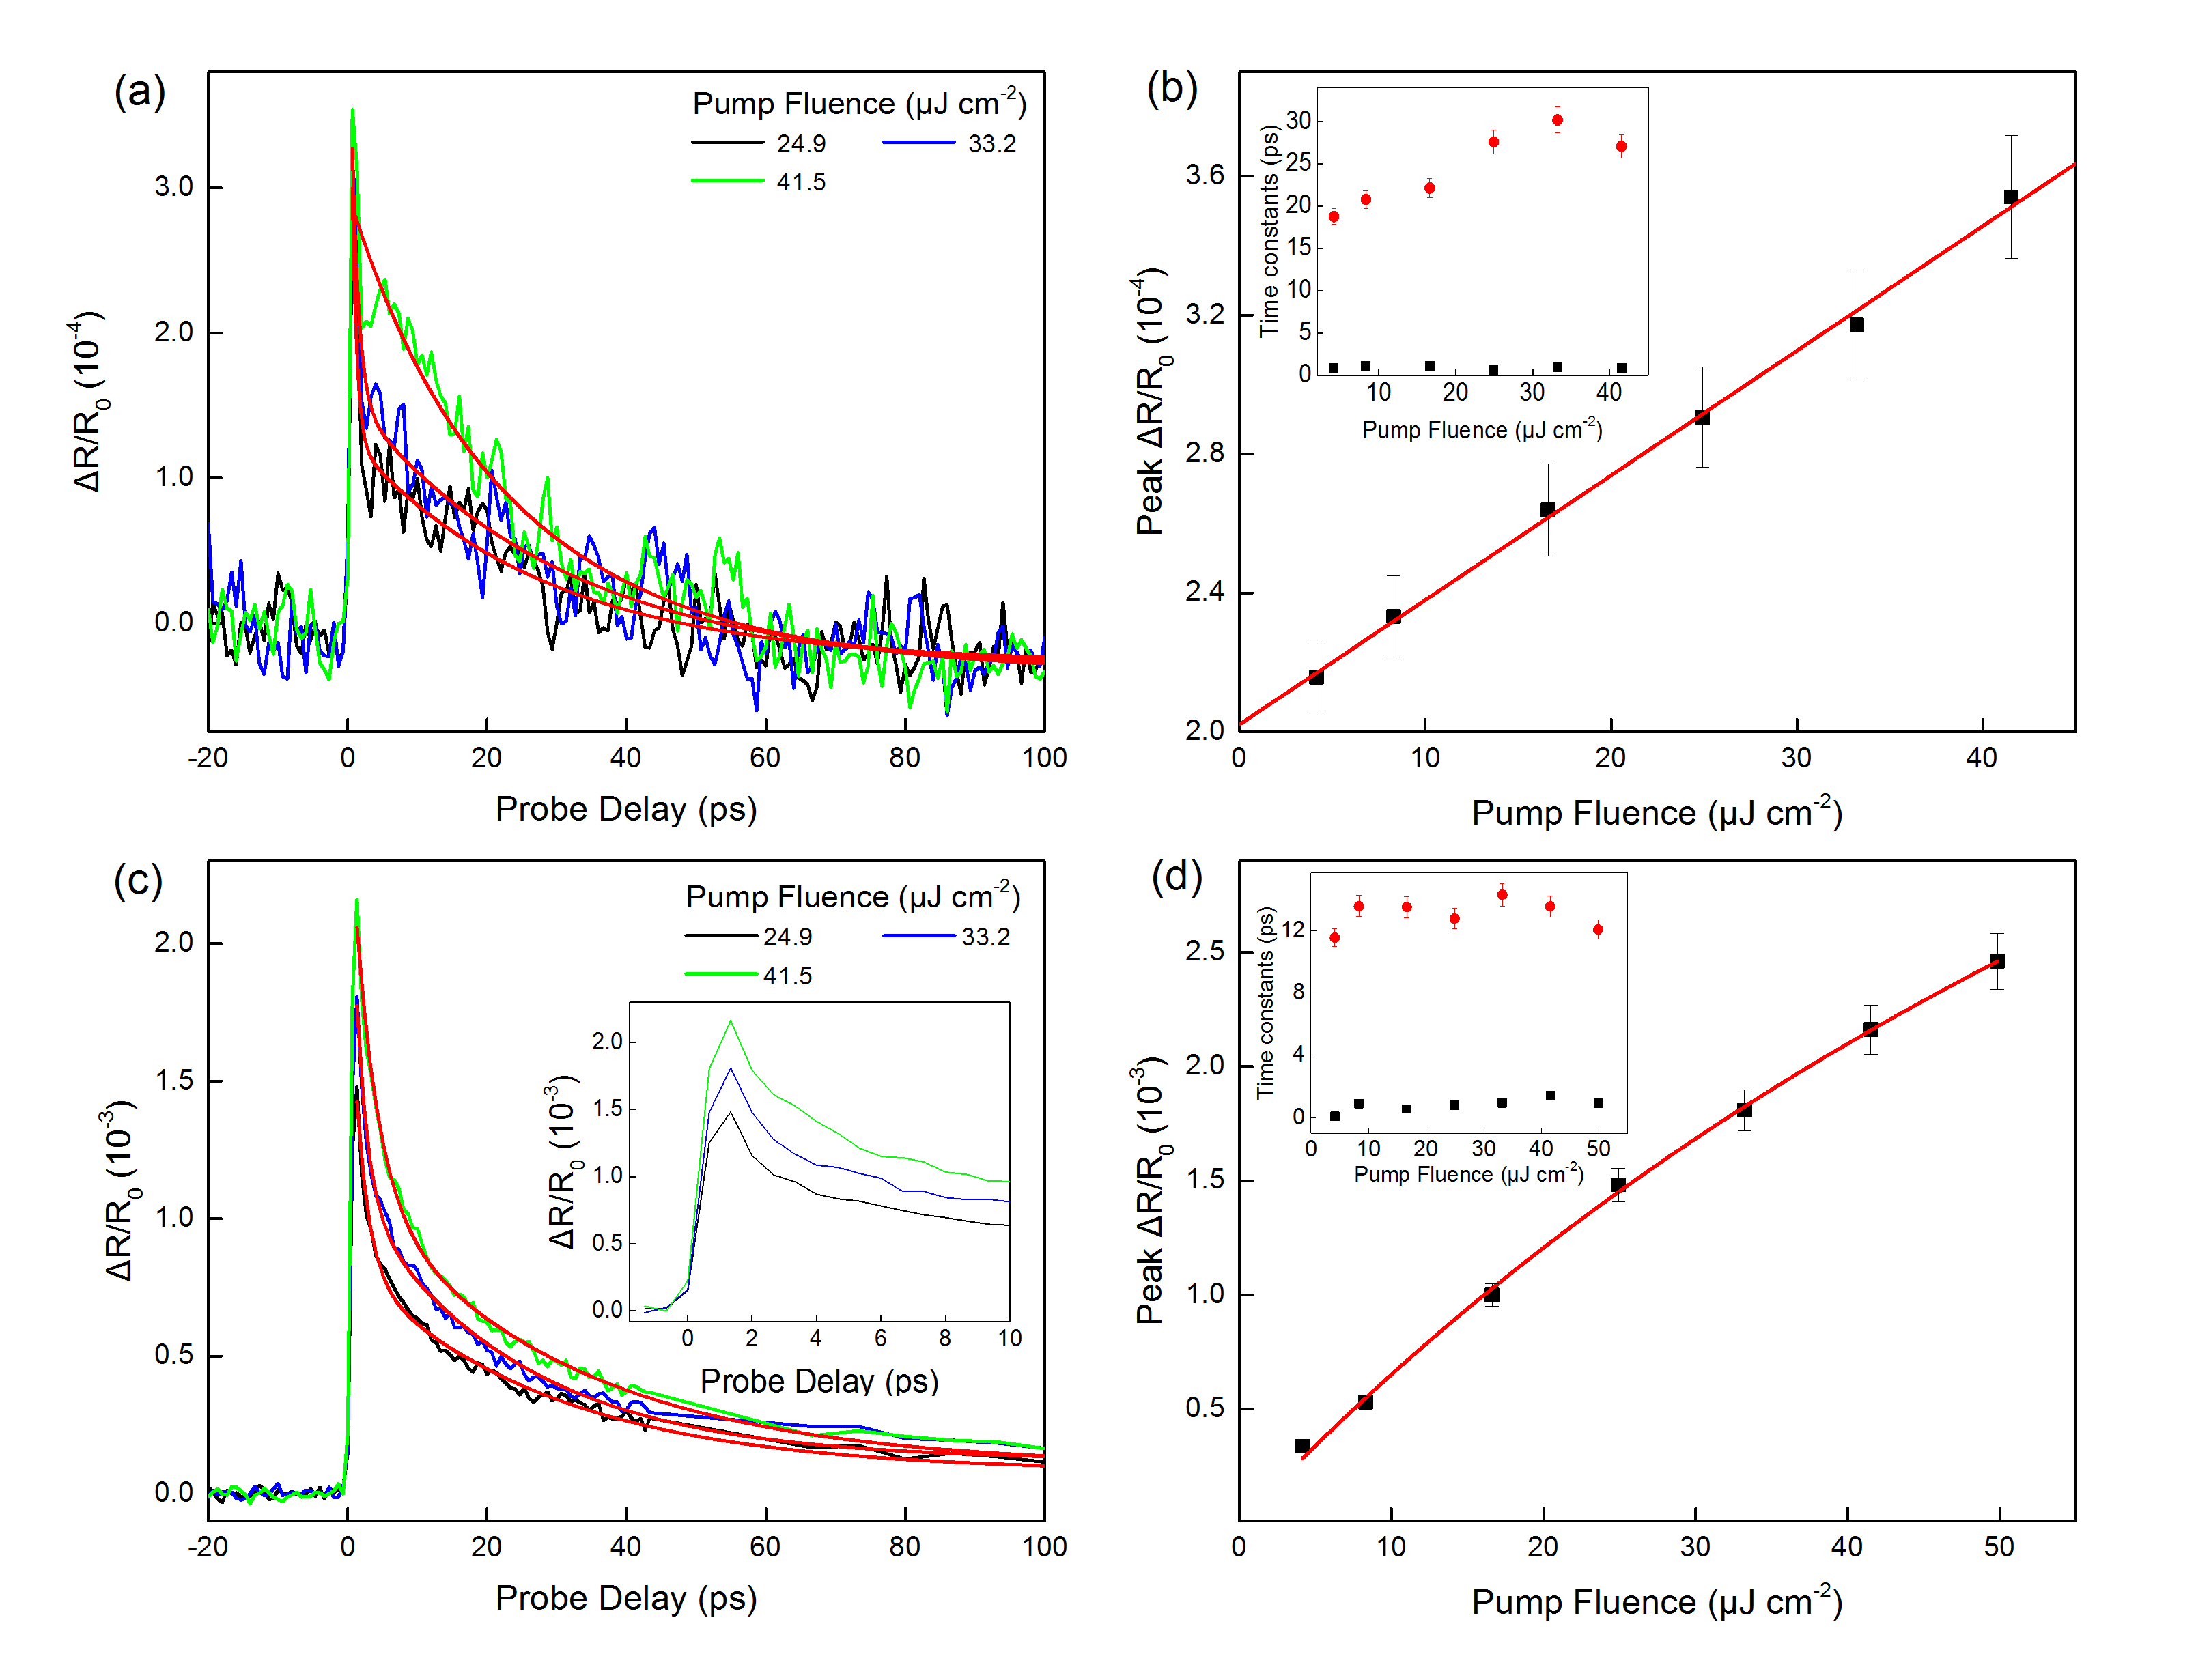
\includegraphics[width=14cm]{dynamics.jpg}
  \caption{(a) Differential reflection signals measured with 410-nm pump and 820-probe pulses from a 1L MoSe$_2$ flake. Black, blue and green curves are signals with pump fluences of 24.9, 33.2, 41.5 $\mu$J cm$^{-2}$, respectively. Red curves are bi-exponential decay fits. (b) Peak differential reflection signal from 1L MoSe$_2$ as a function of the pump fluence. The inset shows the two decay constants as a function of the pump fluence. The red line is a linear fit. (c) Same as (a), but from the 2L-In$_2$Se$_3$/1L-MoSe$_2$ heterostructure. The inset shows the same signals but in a smaller range of the probe delay. (d) Peak differential reflection signal from the 2L-In$_2$Se$_3$/1L-MoSe$_2$ heterostructure. The red line is the fit (see text). The two decay constants are summarized in the inset.}
    \label{fig:dynamics}
\end{figure*}

Study of photocarrier dynamics in 2L-In$_2$Se$_3$/1L-MoSe$_2$ heterostructures can provide further evidence on its type-I band alignment, and provide information on the interlayer energy transfer from In$_2$Se$_3$ to MoSe$_2$, as illustrated in Figure \ref{fig:alignment}(a). We preformed transient absorption measurements in reflection geometry with the setup shown in Figure \ref{fig:tam}. We started with the 1L MoSe$_2$ sample. A tightly focused pump pulse of 410 nm injects photocarriers. The differential reflection (D R / R0) of a 820-nm probe pulse was detected as a function of the probe delay (defined as the arrival time of the probe pulse at the sample, with respect to the pump pulse). The probe wavelength is near the PL peak of the sample, for efficient detection of the photocarriers \cite{afm271604509}.  The results are shown in Figure \ref{fig:dynamics}(a). The decay of the signal can be fit by bi-exponential function, as shown by the red curves in Figure \ref{fig:dynamics}(a). The two time constants are summarized in the inset of Figure \ref{fig:dynamics}(b).  The fast process of 0.9 ps has a weight of about 70 \%. This process has been previously observed in TMDs and has been attributed to the exciton formation process \cite{nanoscale811681,jap120124306,nl171455}. The slow process of 24 ps can be attributed to exciton recombination in 1L MoSe$_2$. Figure \ref{fig:dynamics}(b) shows the peak signal as a function of the pump fluence. The linear dependence confirms that the signal is proportional to the photocarrier density.

These measurements were repeated with the 2L-In$_2$Se$_3$/1L-MoSe$_2$ heterostructure, under the same experimental conditions. The results are shown in Figure \ref{fig:dynamics}(c). Similarly, the decay is fit by bi-exponential functions (red curves), with two time constants shown in the inset of Figure \ref{fig:dynamics}(d). The fast and slow processes have weights of about 60 \% and 40 \%, respectively. Comparing the 1L MoSe$_2$, the magnitude of the signal is about 7 times higher. Since the probe mainly monitors the photocarriers in MoSe$_2$, the enhancement of the signal can only come from the photocarriers that were injected in In$_2$Se$_3$ and subsequently transferred to MoSe$_2$. If the band alignment was type-II, as shown in Figure \ref{fig:alignment}(b), only holes would transfer. These transferred holes would have a very long lifetime in MoSe$_2$, since their recombination with electrons (that are in the In$_2$Se$_3$ layer) was greatly suppressed by their spatial separation. However, we observed a similar (slightly shorter) decay time of the signal in the heterostructure. This shows that the holes transferred have a short lifetime that is comparable to photocarriers injected in 1L MoSe$_2$. Hence, we can conclude that electrons injected in In$_2$Se$_3$ also transfer to MoSe$_2$, and that the band alignment is type-I.

Since both electrons and holes injected in In$_2$Se$_3$ transfer to MoSe$_2$, there is no net charge transfer. The overall process is an energy transfer process. A closer look at the rising part of the signal, as shown in the inset of Figure \ref{fig:dynamics}(c), indicates that the signal reaches a peak on a time scale that is close to the instrument response time. Hence, the transfer of energy from 2L In$_2$Se$_3$ occurs on an ultrafast time scale of a fraction of 1 ps at most. The energy transfer can be achieve by two mechanisms, Fr{\"o}ster-type and Dexter-type energy transfer. The former occurs {\it via} nonradiative dipole-dipole coupling of the two layers: An electron-hole pair (or exciton) in the first layer recombines nonradiatively, transferring the energy for the excitation of an electron-hole pair (or exciton) in the second layer \cite{cr1051491}. The latter involves sequential or simultaneous transfer of both electrons and hole  \cite{jcp21836,jpcb1081537}. From the experiments, we are unable to reveal which mechanism is responsible for the observed transfer, since both mechanisms have the same final result.

Finally, the slightly shorter lifetime of excitons in the heterostructure can be attributed to additional contributions of from exciton-exciton annihilation. Under the same excitation pump fluence, the signal from the heterostructures is about 7 times larger than 1L MoSe$_2$. This suggests that the exciton density in the MoSe$_2$ layer of the heterostructure sample is 7 times higher than 1L MoSe$_2$ sample. It has been generally observed in TMDs that at high densities exciton-exciton can induce shorter carrier lifetimes \cite{b89125427,nl145625,nanoscale77402,nm14889}. Indeed, we observe a saturation effect in the heterostructures, where the peak signal shows a sub-linear dependence on the pump fluence, as shown in Figure \ref{fig:dynamics}(d). The data can be fit by a saturation model, $\Delta R / R_0 \propto F / (F + F_s)$, as shown by the red curve, with the saturation fleunce of $F_s = 11.4~ \mu J~cm^{2}$.

\section{Conclusion}

In summary, we found that CVD-grown heterostructures of 2L-$\alpha$-In$_2$Se$_3$/1L-MoSe$_2$ have a type-I band alignment, with both the CBM and the VBM located in MoSe$_2$. This conclusion is supported by several experimental findings, such as the lack of PL quenching and similar exciton lifetimes in the heterostructure. The energy transfer from In$_2$Se$_3$ to MoSe$_2$ was found to be highly efficient, from the enhanced differential reflection signal from the heterostructure with an ultrashort rising time. We also found that bulk-like In$_2$Se$_3$ forms type-II band alignment with 1L MoSe$_2$, with efficient interlayer charge transfer. These findings suggest that $\alpha$-In$_2$Se$_3$ ultrathin layers can be effectively integrated with other TMD 1Ls for novel optoelectronic applications, with the capability of band alignment control by thickness.




%%%%%%%%%%%%%%%%%%%%%%%%%%%%%%%%%%%%%%%%%%%%%%%%%%%%%%%%%%%%%%%%%%%%%
%% The "Acknowledgement" section can be given in all manuscript
%% classes.  This should be given within the "acknowledgement"
%% environment, which will make the correct section or running title.
%%%%%%%%%%%%%%%%%%%%%%%%%%%%%%%%%%%%%%%%%%%%%%%%%%%%%%%%%%%%%%%%%%%%%
\begin{acknowledgement}

The authors thank the financial support of the National Key R\&D Program of China
(2016YFA0202302), MOST of China (2016YFA0200602), the National Natural Science Foundation of China (61335006, 61527817, 61378073, 11474260, 11504364), Initiative Postdocs Supporting Program of China (BX201600013), General Financial Grant from the China Postdoctoral Science Foundation (2017M610756), Overseas Expertise Introduction Center for Discipline Innovation, 111 Center of China, and National Science Foundation of USA (DMR-1505852). 

\end{acknowledgement}

%%%%%%%%%%%%%%%%%%%%%%%%%%%%%%%%%%%%%%%%%%%%%%%%%%%%%%%%%%%%%%%%%%%%%
%% The same is true for Supporting Information, which should use the
%% suppinfo environment.
%%%%%%%%%%%%%%%%%%%%%%%%%%%%%%%%%%%%%%%%%%%%%%%%%%%%%%%%%%%%%%%%%%%%%


%%%%%%%%%%%%%%%%%%%%%%%%%%%%%%%%%%%%%%%%%%%%%%%%%%%%%%%%%%%%%%%%%%%%%
%% The appropriate \bibliography command should be placed here.
%% Notice that the class file automatically sets \bibliographystyle
%% and also names the section correctly.
%%%%%%%%%%%%%%%%%%%%%%%%%%%%%%%%%%%%%%%%%%%%%%%%%%%%%%%%%%%%%%%%%%%%%

\bibliography{literature}

%%%%%%%%%%%%%%%%%%%%%%%%%%%%%%%%%%%%%%%%%%%%%%%%%%%%%%%%%%%%%%%%%%%%%
%% The "tocentry" environment can be used to create an entry for the
%% graphical table of contents.
%%%%%%%%%%%%%%%%%%%%%%%%%%%%%%%%%%%%%%%%%%%%%%%%%%%%%%%%%%%%%%%%%%%%%


\end{document}
